\addcontentsline{toc}{chapter}{Занятие 4. Оценка максимального правдоподобия}
\chapter*{Занятие 4. Оценка максимального правдоподобия}

\addcontentsline{toc}{section}{Контрольные вопросы и задания}
\section*{Контрольные вопросы и задания}

\subsubsection*{Как построить оценку максимального правдоподобия?}

Плотность распределения выборки $\left( X_1, \dotsc, X_n \right) $ имеет вид
$$L \left( \vec{X}, \theta \right) =
  \prod \limits_{k = 1}^n p \left( X_k, \theta \right),$$
как плотность вектора с независимыми координатами.
$L \left( \vec{X}, \theta \right) $ --- функция правдоподобия.

Оценка максимаьлного правдоподобия $ \hat{ \theta }$ --- такое значение параметра $ \theta $,
при котором функция правдоподобия достикает своего максимального значения
$ \hat{ \theta } =
  \underset{ \theta }{argmax} L \left( \vec{X}, \theta \right) $.

\subsubsection*{Сформулируйте свойства оценки максимального правдоподобия.}

Оценка максимального правдоподобия, как правило, сильно состоятельная.

\addcontentsline{toc}{section}{Аудиторные задачи}
\section*{Аудиторные задачи}

\subsubsection*{4.3}

\textit{Задание.}
Постройте оценку максимального правдоподобия векторного параметра $ \left( a, \sigma^2 \right) $
нормального распределения.

\textit{Решение.} Выборка $x_1, \dotsc, x_n \sim N \left( a, \sigma^2 \right) $.
Сейчас $ \theta $ будет векторным параметром, состоящим из двух элементов: $a, \sigma^2$.

Плотность имеет вид
$$p \left( x \right) =
  \frac{1}{ \sqrt{2 \pi } \sigma } \cdot e^{- \frac{ \left( x - a \right)^2}{2 \sigma^2}}.$$

Произведение этих плотностей даёт
$$L \left( \vec{x}, a, sigma^2 \right) =
  \frac{1}{ \left( 2 \pi \right)^{ \frac{n}{2}} \sigma^2}
  \cdot e^{- \frac{1}{2 \sigma^2} \cdot \sum \limits_{i = 1}^n \left( x_i - a \right)^2}.$$
Обозначим $ \sigma^2 = \sigma^*$, чтобы было удобней брать производную
$$ \frac{1}{ \left( 2 \pi \right)^{ \frac{n}{2}} \sigma^2}
  \cdot e^{- \frac{1}{2 \sigma^2} \cdot \sum \limits_{i = 1}^n \left( x_i - a \right)^2} =
  \frac{1}{ \left( 2 \pi \right)^{ \frac{n}{2}} \left( \sigma^* \right)^{ \frac{n}{2}}} \cdot
  e^{- \frac{1}{2 \sigma^*} \cdot \sum \limits_{i = 1}^n \left( x_i - a \right)^2}.$$

Поскольку есть экспонента, стоит брать логарифм
$$l \left( \vec{x}, a, \sigma^* \right) =
  ln L \left( \vec{x}, a, \sigma^* \right) =
  - \frac{n}{2} \cdot ln \left( 2 \pi \sigma^* \right) -
  \frac{1}{2 \sigma^*} \sum \limits_{i = 1}^n \left( x_i - a \right)^2.$$
Распишем логарифм произведения через сумму логарифмов
$$- \frac{n}{2} \cdot ln \left( 2 \pi \sigma^* \right) -
  \frac{1}{2 \sigma^*} \sum \limits_{i = 1}^n \left( x_i - a \right)^2 =
  - \frac{n}{2} \cdot ln \left( 2 \pi \right) -
  \frac{n}{2} \cdot ln \sigma^* -
  \frac{1}{2 \sigma^*} \sum \limits_{i = 1}^n \left( x_i - a \right)^2.$$

Берём производную
$$ \frac{ \partial }{ \partial \sigma^*} l =
  - \frac{n}{2} \cdot \frac{1}{ \sigma^*} +
  \frac{1}{2 \left( \sigma^* \right)^2} \sum \limits_{i = 1}^n \left( x_i - a \right)^2 =
  0.$$

Теперь надо по $a$ продифференцировать и тоже приравнять к нулю
$$ \frac{ \partial }{ \partial a} l =
  \frac{1}{ \sigma^*} \sum \limits_{i = 1}^n \left( x_i - a \right) =
  0 =
  \frac{n \overline{X} - na}{ \sigma^*}.$$

Распишем сумму в явном виде
$ \left( x_1 - a \right) + \left( x_2 - a \right) + \dotsc + \left( x_n - a \right) =
  0$.

Отсюда
$$a =
  \frac{1}{n} \sum \limits_{i = 1}^n x_i.$$

Оценка равна $ \hat{a} = \overline{x}.$

Тогда оценка второго параметра равна
$$ \hat{ \sigma^*} =
  \frac{1}{n} \sum \limits_{i = 1}^n \left( x_i - \overline{x} \right)^2.$$

Проверили только необходимое условие для максимума.
Теперь нужно проверить достаточность.

Имеем матрицу $n \times n$.
Матрица положительно определена тогда и только тогда, когда каждый минор положительный.
Матрица отрицательно определена тогда и только тогда, когда каждый минор отрицательный.

$$ \begin{bmatrix}
  \frac{ \partial^2}{ \partial a^2} & \frac{ \partial^2}{ \partial a \partial \sigma^*} \\
  \frac{ \partial^2}{ \partial a \partial \sigma^*} & \frac{ \partial^2}{ \partial \left( \sigma^* \right)^2}
\end{bmatrix}.$$

Найдём последний элемент матрицы
$$ \frac{ \partial^2}{ \partial \left( \sigma^* \right)^2} l =
  \frac{n}{2 \left( \sigma^* \right)^2} -
  \frac{1}{ \left( \sigma^* \right)^3} \cdot \sum \limits_{i = 1}^n \left( x_i - a \right)^2.$$

Найдём смешанную производную
$$ \frac{ \partial^2}{ \partial a \partial \sigma^*} l =
  - \sum \limits_{i = 1}^n \left( x_i - a \right) \cdot \frac{1}{ \left( \sigma^* \right)^2} =
  \frac{n \overline{x} - na}{ \left( \sigma^* \right)^2}.$$

Найдём первый элемент матрицы
$$ \frac{ \partial^2}{ \partial a^2} l =
  - \frac{n}{ \sigma^*}.$$

Теорема Шварца.
Если
$$ \exists \frac{ \partial^2 f}{ \partial x \partial y}, \,
  \frac{ \partial^2 f}{ \partial y \partial x}$$
и они непрерывны в точке $ \left( x_0, y_0 \right) $, то они совпадают в этой точке.

Первый определитель строго отрицательный.

Второй определитель
$$M_2 =
  - \frac{n^2}{2 \left( \sigma^* \right)^3} +
  \frac{n}{ \left( \sigma^* \right)^4} \cdot \sum \limits_{i = 1}^n \left( x_i - a \right) -
  \frac{n}{ \left( \sigma^* \right)^4} \cdot \left( \overline{x} - a \right)^2.$$
Последнее слагаемое равно нулю.
Нужно проверять это значение в точке $ \hat{a} = \overline{x}$.
Имеем
\begin{equation*}
  \begin{split}
    - \frac{n^2}{2 \left( \sigma^* \right)^3} +
    \frac{n}{ \left( \sigma^* \right)^4} \cdot \sum \limits_{i = 1}^n \left( x_i - a \right) -
    \frac{n}{ \left( \sigma^* \right)^4} \cdot \left( \overline{x} - a \right)^2 = \\
    = - \frac{n}{ \left( \sigma^* \right)^3} \cdot
    \left( \frac{n}{2} - \frac{1}{ \sigma^*} \cdot
    \sum \limits_{i = 1}^n \left( x_i - a \right) \right) >
    0.
  \end{split}
\end{equation*}

Нужно проверить в точке $ \sigma^* = \hat{ \sigma }$.
Имеем
$$ \frac{n}{2} <
  \frac{ \sum \limits_{i = 1}^n \left( x_i - a \right)^2}{ \sigma^*}.$$

Отсюда выражаем значение оценки
$$ \sigma^* =
  \hat{ \sigma } =
  \frac{1}{n} \sum \limits_{i = 1}^n \left( x_i - \overline{x} \right).$$
Следовательно,
$$ \frac{n}{2} < n,$$
то есть $M_2 < 0$.
По критерию Сильвестра $ \hat{A} < 0$ тогда и только тогда,
когда $ \left( \hat{a}, \hat{ \sigma^*} \right) $ --- точка максимума.

\subsubsection*{4.5}

\textit{Задание.}
Постройте оценку максимального правдоподобия параметра $ \theta $ показательного распределения.

\textit{Решение.}
$p \left( x, \theta \right) =
  \theta e^{- \theta x} \cdot \mathbbm{1} \left\{ x \geq 0 \right\} $.

Нужно найти функцию правдобоподия как произведение плотностей
$L \left( \vec{x}, \theta \right) =
  \theta^n \cdot e^{-n \theta \sum \limits_{i = 1}^n x_i} \cdot
  \mathbbm{1} \left\{ \vec{x} \in \left[ 0, + \infty \right)^n \right\} $.
Предполагаем, что все $x_i \geq 0$, то есть индикатор можно отбросить.
Если какой-то элемент выборки сильно отрицательный,
то не имеет смысла говорить о равномерном распределении.
Если какой-то элемент выборки близок к нулю и при этом отрицательный, то на него повлияла ошибка,
и его не учитываем
$$ \theta^n \cdot e^{-n \theta \sum \limits_{i = 1}^n x_i} \cdot
  \mathbbm{1} \left\{ \vec{x} \in \left[ 0, + \infty \right)^n \right\} =
  \theta^n e^{-n \theta \sum \limits_{i = 1}^n x_i}.$$

Удобнее будет рассмотреть
$$ln L \left( \vec{x}, \theta \right) =
  l \left( \theta \right) =
  - \theta \sum \limits_{i = 1}^n x_i + n ln \theta.$$

Нужно взять производную и приравнять к нулю
$$ \frac{ \partial }{ \partial \theta } l \left( \theta \right) =
  - \sum \limits_{i = 1}^n x_i + \frac{n}{ \theta } =
  0.$$

Переносим сумму вправо
$$ \frac{n}{ \theta } =
  \sum \limits_{i = 1}^n x_i.$$

Получаем оценку
$$ \hat{ \theta } =
  \frac{n}{ \sum \limits_{i = 1}^n x_i}.$$
Выразим через выборочное среднее
$$ \frac{n}{ \sum \limits_{i = 1}^n x_i} =
  \frac{1}{ \overline{X}}.$$
Остаётся проверить, что $ \hat{ \theta }$ будет действительно максимумом функции $l$.
Нужно найти вторую производную
$$ \frac{ \partial^2}{ \partial \theta^2} l \left( \theta \right) =
  - \frac{n}{ \theta^n} <
  0.$$
Отсюда следует, что фунция выпуклая ввекх, соответственно это точка максимума.

\subsubsection*{4.6}

\textit{Задание.}
Постройте оценку максимального правдоподобия параметра $ \theta > 0$
равномерного распределения на отрезке $ \left[ 0, \theta \right] $.

\textit{Решение.}
Плотность равномерного распределения на отрезук $ \left[ 0, \theta \right] $ имеет вид
$$p_{ \theta } \left( x \right) =
  \frac{ \mathbbm{1} \left\{ x \in \left[ 0, \theta \right] \right\} }{ \theta }.$$
По этой плотности строим функцию правдоподобия
$$L \left( \vec{x}, \theta \right) =
  \frac{ \mathbbm{1} \left\{ \vec{x} \in \left[ 0, \theta \right]^n \right\} }{ \theta^n} =
  \frac{ \mathbbm{1} \left\{ \min \limits_i x_i \geq 0, \, \max \limits_i x_i \leq \theta \right\} }{ \theta^n}.$$
Если какой-то элемент выборки сильно отрицательный,
то не имеет смысла говорить о равномерном распределении, если близок к нулю,
то на него повлияла ошибка, и его не учитываем
$$ \frac{ \mathbbm{1} \left\{ \min \limits_i x_i \geq 0, \, \max \limits_i x_i \leq \theta \right\} }{ \theta^n} =
  \frac{ \mathbbm{1} \left\{ \max \limits_i x_i \leq \theta \right\} }{ \theta }.$$

Нарисуем график получившейся функции как функции от $ \theta $ (рис. \ref{fig:46}).

\begin{figure}[h!]
  \centering
  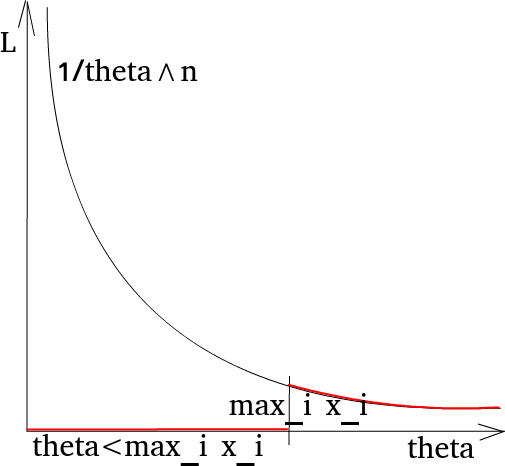
\includegraphics[width=.4\textwidth]{./pictures/4_6.png}
  \caption{График функции $L \left( \theta \right) $}
  \label{fig:46}
\end{figure}

Точка максимума такой функции --- это $ \max \limits_i x_i$.

Значит, $ \hat{ \theta } = \max \limits_{1 \leq i \leq n} x_i$.

\addcontentsline{toc}{section}{Домашнее задание}
\section*{Домашнее задание}
